%We will now discuss  an example demonstrating the need to describe attenuation in specifications.
\emph{Attenuation} is the ability to provide to third party objects \emph{restricted}  access to an object's functionality. This is usually achieved through the introduction of an intermediate object. While such intermediate objects are a common programming practice, 
the term was coined, and the practice  was studied in detail in the object capabilities literature \cite{MillerPhD}. 

Specifications for attenuation for the DOM were proposed in \cite{dd}. 
In this section we revisit that example and also argue that compared with the specification in \cite{dd}, our specification xxxx.

This example deals with a tree of DOM nodes: Access to a DOM node gives access to all its parent and children nodes, and the ability to modify the node's properties. However, as the top nodes of the tree usually contain privileged information, while the lower nodes contain less crucial information, such as xxxx, we want to be able to limit  access given to third parties to only the lower part of the DOM tree. We do this through a \prg{Wrapper}, which has a field \prg{node} pointing to a \prg{Node}, and a field \prg{height} which restricts the range of \prg{Node}s which may be modified through the use of the particular \prg{Wrapper}. Namely, when you hold a \prg{Wrapper}  you can modify the \prg{property} of all the descendants of the    \prg{height}-th ancestors of the \prg{node} of that particular \prg{Wtrapper}.  It is not difficult to write such a \prg{Wrapper}; a possible implementation  appears in Figure \ref{fig:DOM} in appendix \ref{DOM:traditional}.


In Figure \ref{fig:WrapperUse} we show an example of the use of  \prg{Wrapper} objects to attenuate the use of \prg{Node}s\footnote{SD: Is that a good sentence?}  The function \prg{usingWrappers} takes as parameter an object of unknown provenance, here called \prg{unknwn}. On lines 2-7 we create  a tree consisting of nodes \prg{n1}, \prg{n2}, ... \prg{n6}, depicted as blue circles on the   right-hand-side of the Figure. On line 8 we create a wrapper of \prg{n5} with height \prg{1}. This means that the wrapper \prg{w} may be used to modify \prg{n3}, \prg{n5} and \prg{n6} (\ie the objects in the green triangle), while it cannot be used to modify \prg{n1}, \prg{n2}, and \prg{4} (\ie the objects within the blue triangle). 
On line 8 we call a  function named \prg{untrusted} on the \prg{unknown} object, and pass \prg{w} as   argument. 

\begin{figure}[htb]
\begin{tabular}{llll}
\ \ &
\begin{minipage}{0.45\textwidth}
\begin{lstlisting}
method usingWrappers(unknwn){
   n1=Node(null,"fixed"); 
   n2=Node(n1,"robust"); 
   n3=Node(n2,"const"); 
   n4=Node(n3,"volatile");
   n5=Node(n4,"variable");
   n6=Node(n5,"ethereal");
   w=Wrapper(n5,1);
   
   unknwn.untrusted(w);
   
   assert n2.property=="robust" 
   ...
}
\end{lstlisting}
\end{minipage}
& & 
\begin{minipage}{0.75\textwidth}
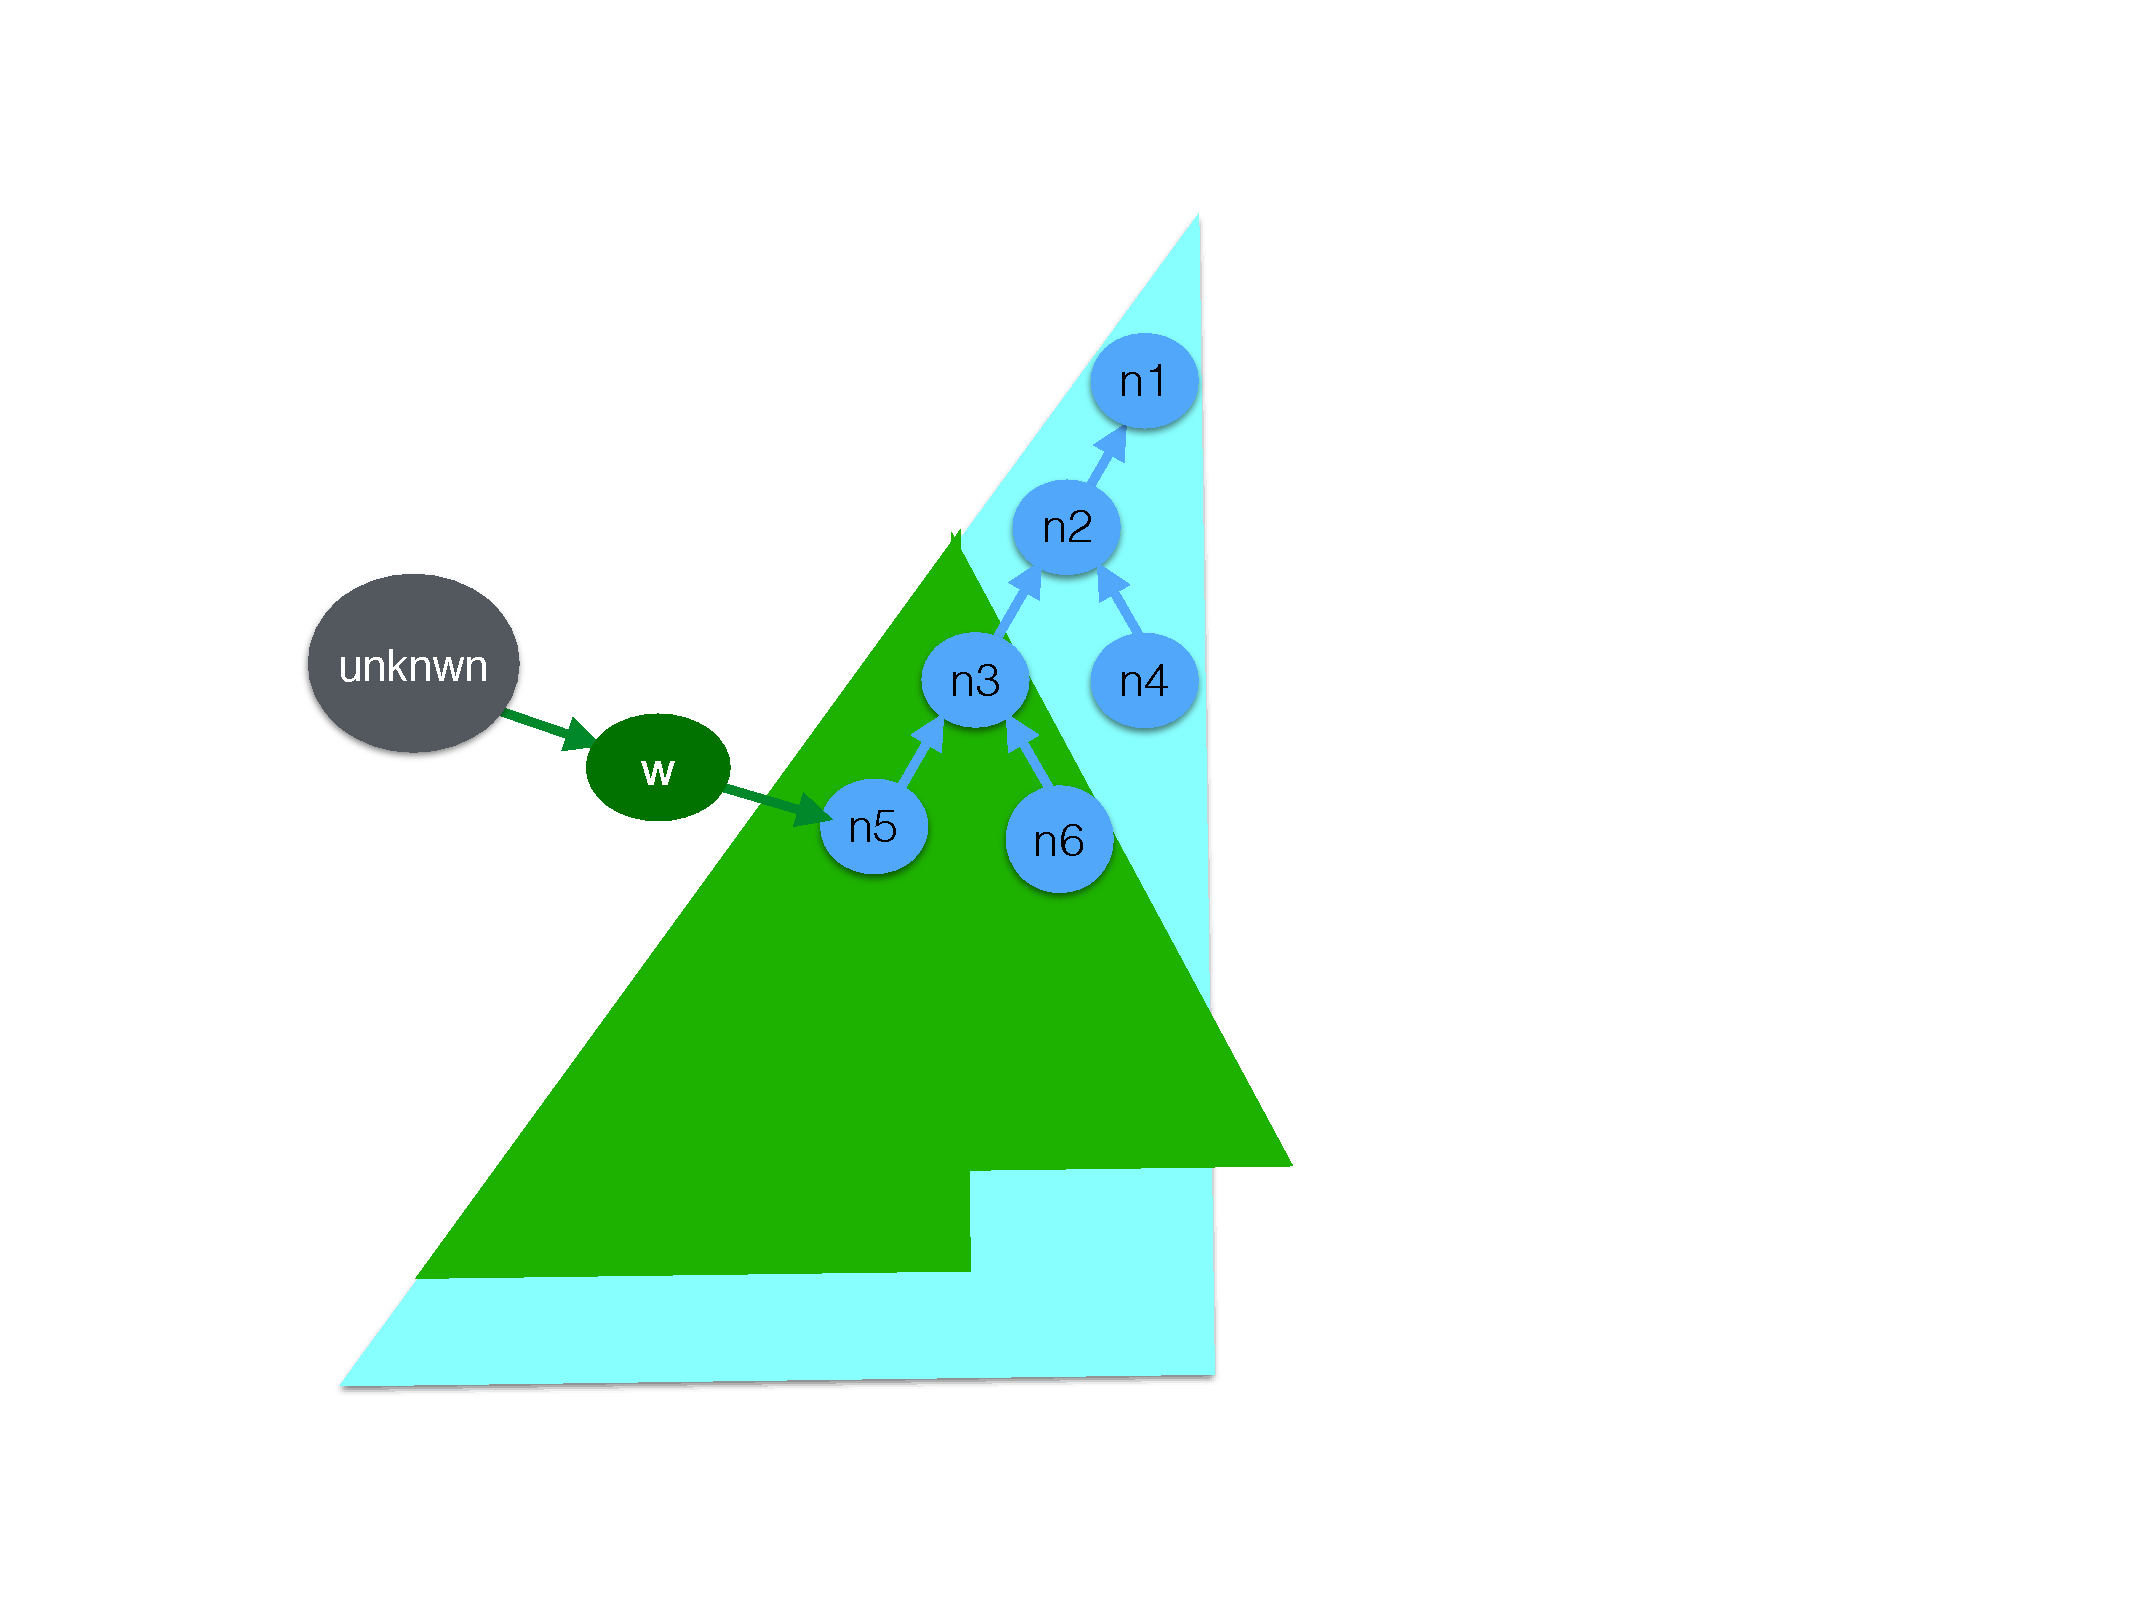
\includegraphics[width=\linewidth, trim=145  320 60 105,clip]{diagrams/DOM.pdf}
% x y z w
% y seems to eat up the bollom
% y=320 is good
% x eats space from left, if you increase it the diagram decreases from left
% w eats space from top, if you increase it the diagram decreases from top
% w=100 is good
%\includegraphics[page=3, width=\linewidth, trim=150  270 40 150, clip]{diagrams/snmalloc.pdf}\sdcomment{I think we need to change the diagram so that it says small slab.}
\strut \\
\strut \\

\end{minipage}
\end{tabular}
 \vspace*{-4.5mm}
\caption{\prg{Wrapper}s protecting \prg{Node}s }
\label{fig:WrapperUse}
\end{figure}

Even though we know nothing about the \prg{unknown} object or its \prg{untrusted} function, and even though the call gives to \prg{unknown}  access to \prg{w}, which in turn has transitive access to all  \prg{Node}-s in the tree, 
we know that %the call to the \prg{untrusted} function is guaranteed not to 
line 100 will not affect the   \prg{property} fields of the nodes \prg{n1}, \prg{n2}, and \prg{n4}. 
Thus, the assertion on line 12 is guaranteed to succeed. 
The question is how do we specify \prg{Wrapper}, so as to be able to make such an argument. %prove this assertion.

A  specification of the class \prg{Wrapper} 
in the traditional   style, \eg  \cite{Leavens-etal07} (\cf appendix \ref{DOM:traditional}) consists of pairs of pre- and post- conditions for each of the functions of that class. Each such pair gives a {\em sufficient} condition for some effect to take place: for example the call \prg{w.setProperty(i,prp)} where \prg{i} is smaller than \prg{w.height} is a sufficient condition to  modify   \prg{property} of the \prg{i}-th parent of \prg{w.node}. But we do not know what other ways there may be  to modify a node's  \prg{property}. In other words, we have not specified the \emph{necessary conditions}. \footnote{Shell we say the following, or does it break the flow? \\
Moreover, on line 10 we do not know which functions are called on \prg{w}.}

Instead, in this work, we propose \emph{holistic specifications}, which describe the behaviour of an abstract data type as a hole, taking all possible method calls into account. Such holistic specifications typically describe \emph{necessary conditions} for some effect to take place. In our example:

\begin{quote}
The \emph{necessary} condition for the modification of \prg{nd.property} for some \prg{nd} of class \prg{Node}  is either access to some   \prg{Node} in the same tree, or  access to a \prg{w} of class \prg{Wrapper} where the \prg{w.height}-th parent of \prg{w} is an ancestor of \prg{nd}.
\end{quote}


With such a specification we can prove that the assertion on line 12 will succeed. And, more importantly, we can ensure that all future updates of the \prg{Wrapper} abstract data type will uphold the \emph{protection} of the \prg{Node} data.
%
% Having justified the need for  necessary conditions in specifications, 
%
To give a flavour of \Chainmail, we use it  express the requirement from above:
%  This  gives us the opportunity to  demonstrate primitives for time ($\Future{\_}$) and authority ($\Changes{\_}$ and $\Using {\_} {\_}$).
 % and   more traditional relations between objects ( $\prg{nd}.\prg{parnt}^k\!=\! ...$):
% $\strut$ 
\vspace{.1cm}

\noindent
% \begin{quote}
$\forall \prg{S}:\prg{Set}.\forall \prg{nd}:\prg{Node}.\forall \prg{o}:\prg{Object}.$\\
$[\ \ {\Using{\Future {\Changes {\prg{nd.property}}}}  {\prg{S}}}$ \\
$\strut  \ \ \longrightarrow$\\
$\strut \ \ \ \exists \prg{o}.[\ \prg{o}\in\prg{S}\ \ \wedge\ \ \neg(\prg{o}:\prg{Node})\ \ \wedge\  \ \neg(\prg{o}:\prg{Wrapper})\ \ \ \wedge \  $\\
$ \strut\ \ \  \ \ \ \ \ \ \ \ [\ \exists \prg{nd}':\prg{Node}. \CanAccess{\prg{o}}{\prg{nd}'}\  \ \ \  \vee$\\
$ \strut\ \  \ \  \ \  \ \ \ \ \ \ \ \exists \prg{w}:\prg{Wrapper}.\exists k\!:\!\mathbb{N}.
% $\\ $ \strut \ \ \ \ \ \ \ \ \ \ \ \ \ \ \ \ \  \ \ \
  (\ \CanAccess{\prg{o}}{\prg{w}}  \ \wedge\ \prg{nd}.\prg{parnt}^k\!=\!\prg{w.node}.\prg{parnt}^{\prg{w.height}}) \ \ \ ]\ ]$\\
$ ]$
% \end{quote}

\vspace{.1cm}

\noindent
That is, if  the value of \prg{nd.property} is modified ($\Changes{\_}$) at some future point ($\Future{\_}$) 
and if reaching that future point involves no more objects than those from
set \prg{S} (\ie ${\Using{\_} {\prg{S}}}$), then at least one (\prg{o}) of the objects in \prg{S} is not a \prg{Node} nor a \prg{Wrapper}, and \prg{o} has direct access to some  node ($\CanAccess{\prg{o}}{\prg{nd}'}$), or  to some wrapper \prg{w} and the \prg{w.height}-th parent of \prg{w} is an ancestor of \prg{nd} (that is, $\prg{parnt}^k\!=\!\prg{w.node}.\prg{parnt}^{\prg{w.height}}$).
% It is important to clarify what we mean by ``access''. 
Definitions of these concepts   appear later (Definition \ref{def:valid:assertion}), but  note that our ``access'' is intransitive: $\CanAccess x y$ holds if  either \prg{x} has a field  pointing to \prg{y}, or  \prg{x}  is the receiver and \prg{y} is one of the arguments  in the executing method call.
 
In the next sections we proceed with a formal model of our model. In the appendix we discuss more -- and simpler -- examples.
We chose the DOM for the introduction, in order to give a flavour of the \Chainmail features.
 
